\chapter{Historija lunaparka}

Zabavni parkovi ili lunaparkovi su prostori ispunjeni različitim sadržajima namijenjenim zabavi. Podgrupa zabavnih parkova su tematski parkovi, kod kojih su atrakcije i struktura bazirani na jednoj temi. Prvi tematski parkovi su nastali sredinom dvadesetog stoljeća, među kojima se ističe najpopularniji, Disneyland, otvoren 1955. godine \cite{Global}. Najposjećeniji tematski park na svijetu je Magic Kingdom u Floridi, dio Walt Disney Worlda, kojeg je samo 2019. godine posjetilo preko 20 miliona ljudi \cite{tematski}. Procjenjuje se da na svijetu ima nekoliko hiljada zabavnih parkova, koji ukupno godišnje zarade preko 220 milijardi dolara \cite{900years}. 

Zabavni parkovi su se razvili iz nekoliko starih tradicija, a to su: putujući sajmovi, vrtovi zadovoljstva, te međunarodne izložbe, odnosno svjetski sajmovi. Za razliku od navedenih, zabavni parkovi su trajnog karaktera. Jedan od najranijih poznatih sajmova bio je Bartholomew Fair u Engleskoj, koji je počeo sa radom 1133. godine. Prvi vrtovi zadovoljstva ili zabave nastali su u Europi u 16. stoljeću. Tako su se zvali jer su imali puno atrakcija koje su zabavljale ljude, poput muzike, igara i vožnji. Jedan od njih je i najstariji zabavni park koji je još u funkciji, Bakken u Klampenborgu u Danskoj. Postoji od 1583. godine, a smatra se da su njegovi pojedini dijelovi još stariji \cite{900years}. Još jedan popularan vrt zadovoljstva je Vauxhall Gardens, nastao 1661. godine u Londonu. Često je okupljao ogromni broj ljudi svojim brojnim atrakcijama, kao što su akrobati, baloni vrućeg zraka, koncerti, te vatrometi. Imao je sistem plaćanja ulaza. Iako je isprva bio namijenjen eliti, uskoro je postao mjesto za sve slojeve društva \cite{UKHistorija}. Prater u Beču u Austriji započeo je sa radom kao kraljevsko mjesto za lov 1766. godine. Uskoro su se oko tog mjesta otvorili kafići, te razne atrakcije, što je dovelo do stvaranja zabavnog parka. Danas se u njemu nalazi najduži vrtuljak na svijetu, te je jedan od najbolje ocijenjenih zabavnih parkova svijeta \cite{900years}. 

\begin{figure}[h!]
  \centering
  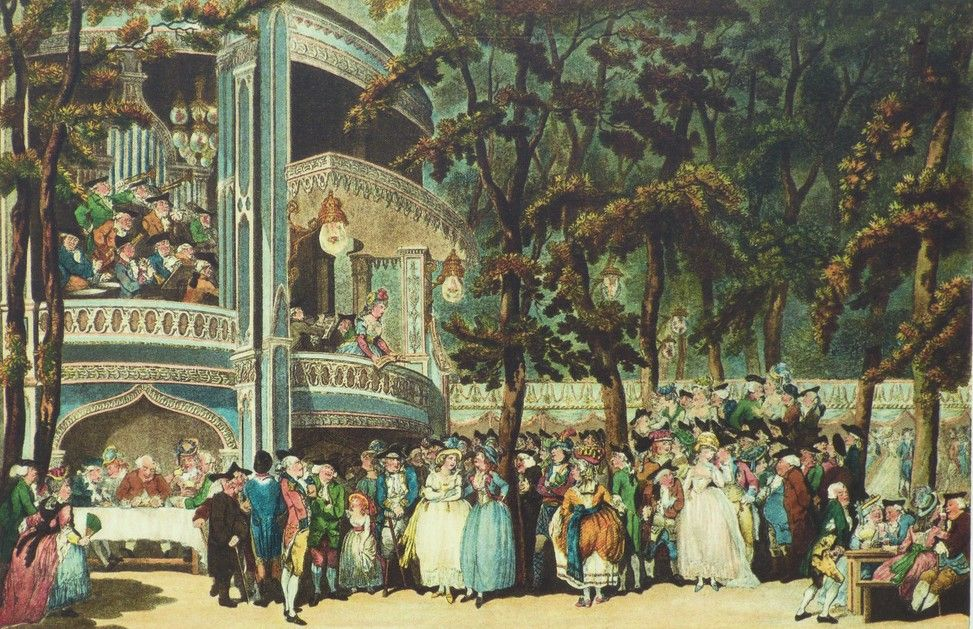
\includegraphics[width=0.7\textwidth]{vauxhall}
  \caption{Vauxhall Gardens \cite{900years}}
  \label{fig:Slika_Vauxhall}
\end{figure}

Svjetski sajmovi utjecali su na razvijanje koncepta trajnog parka namijenenog zabavi. Prvi svjetski sajam počeo je 1851. godine konstrukcijom Kristalne palače u Londonu u Engleskoj. Njegova svrha je bila proslava industrijskog napretka, te je dizajniran za edukaciju i zabavu posjetitelja. Posjetilo ga je 6 miliona ljudi, te je po ugledu na njega organiziran niz svjetskih sajmova širom Europe, a kasnije i Amerike. Svjetska kolumbijska izložba, organizirana 1893. godine u Chicagu u Sjedinjenim Američkim Državama se smatra pretečom modernih zabavnih parkova, s obzirom na brojne sadržaje koje su kasnije svi zabavni parkovi imali, poput vožnji, igara, svjetala, iluzija, te prvog željeznog vrtuljka\cite{worldfairs}. Uskoro su postala popularna različita odmarališta uz rijeke, jezera ili mora, koja su nudila različite zabavne sadržaje za svoje posjetitelje. U njima je izgrađen i prvi voz smrti (eng.\textit{rollercoaster}), izgrađen u Pennsylvaniji u Sjedinjenim Američkim Državama, te najstariji vrtuljak (karusel), izgrađen 1780. godine za princa Wilhelma IX od Hessen-Kassela, te, iako nije funkcionalan, može se vidjeti u Wilhelmsbad Parku u Hanauu u Njemačkoj, rodnom gradu braće Grimm \cite{900years}. 

\begin{figure}[h!]
  \centering
  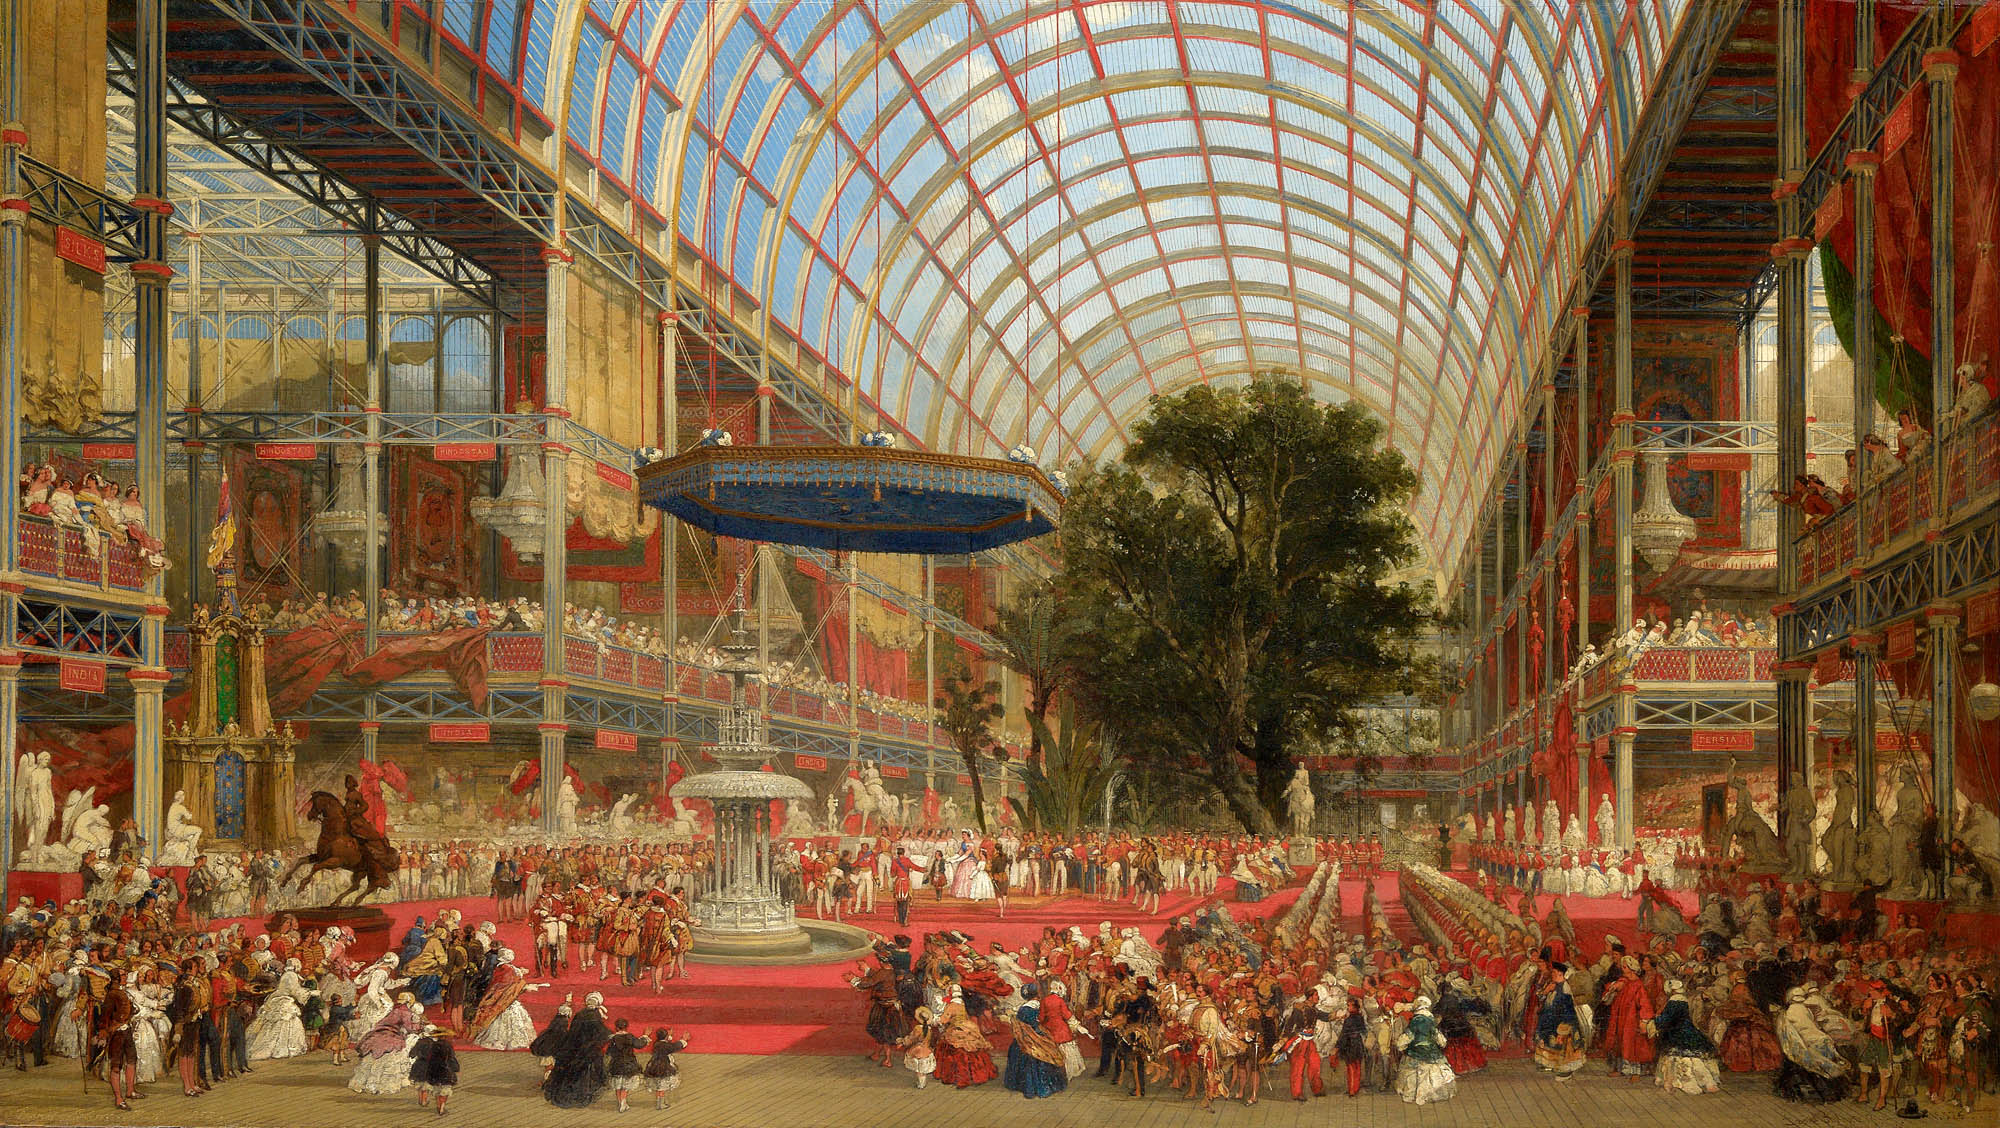
\includegraphics[width=0.7\textwidth]{fair}
  \caption{Prvi svjetski sajam, ulje na platnu od Davida Robertsa \cite{rct}}
  \label{fig:Slika_sajaml}
\end{figure}

Početkom 20. stoljeća, željezničke kompanije su, kako bi ostvarivale profit i vikendom, kad se ljudi manje kreću pošto ne putuju na posao i natrag, počeli otvarati takozvane \textit{trolley} parkove, koji su u početku imali dešavanja poput plesova, koncerata, vatrometa, a kasnije dobili gotovo sve sadržaje koje imaju današnji zabavni parkovi, poput vrtuljaka, vrteški, vozova smrti, i slično, te raznih restorana, vožnji brodovima, bazena, te brojnih drugih zabavnih sadržaja. Smatraju se pretečama današnjih zabavnih parkova. Jedan od najpopularnijih i najuspješnijih bio je Coney Island, pokraj autoputa u Coney Islandu u Brooklynu. Procjenjuje se da je u ovom periodu u Sjedinjenim Američkim Državama bilo između 1500 i 2000 \textit{trolley} parkova. Njihova popularnost se smanjila kad se povećala popularnost automobila \cite{kolica}.

\begin{figure}[h!]
  \centering
  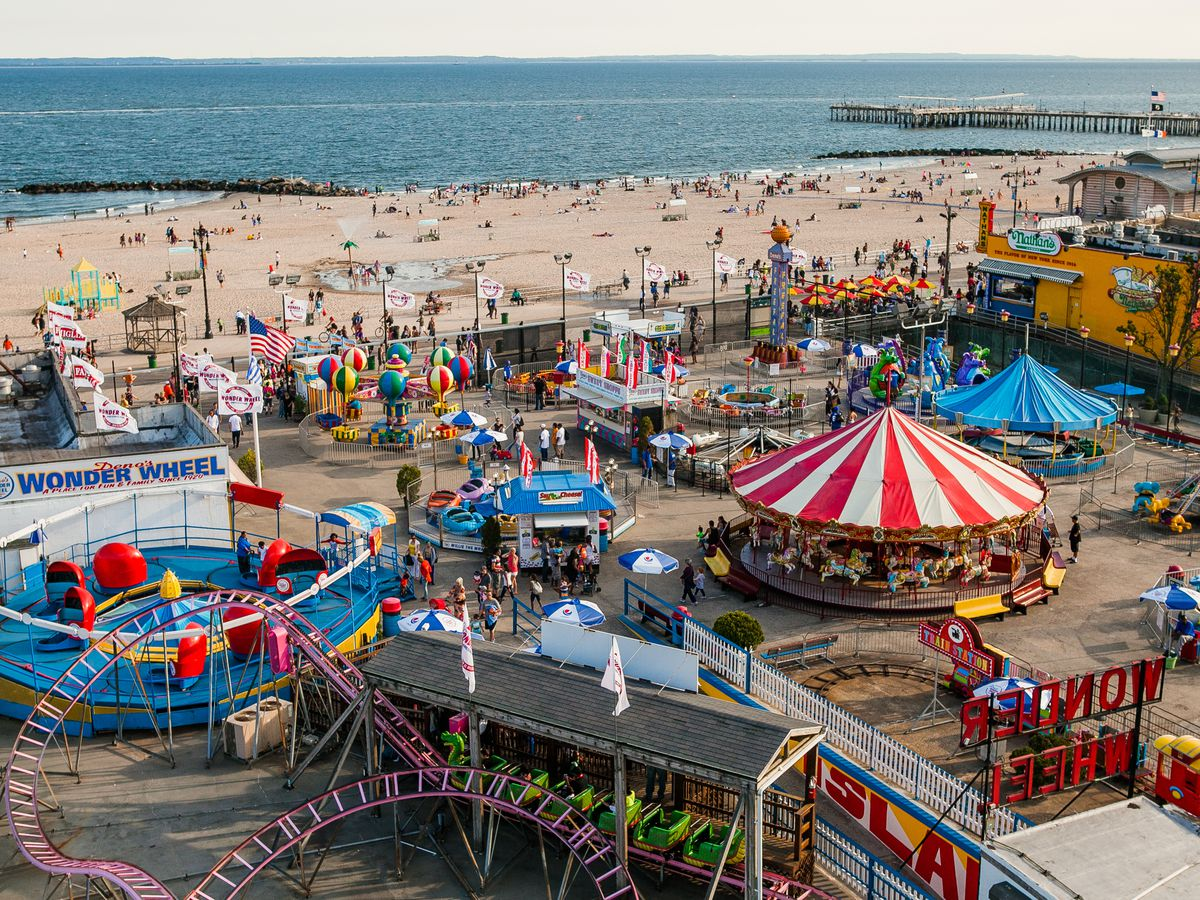
\includegraphics[width=0.7\textwidth]{coney}
  \caption{Coney Island u New Yorku \cite{coney}}
  \label{fig:Slika_Coney}
\end{figure}

Prvo trajno zatvoreno područje namijenjeno zabavi kojim upravlja jedna kompanija osnovano je 1895. godine u Coney Islandu u Brooklynu, a zvalo se Sea Lion Park. To je bio prvi zabavni park u kojem se, osim ulaza, plaćao i pristup pojedinim atrakcijama. Kad mu se 1897. godine pridružio Steeplechase Park, zbog blizine centra sa jako velikim brojem stanovništva, te lakoće pristupa, Coney Island je postao utjelovljenje američkog zabavnog parka. Njegovi dijelovi su bili i Luna Park, te Dreamland \cite{american}. Zbog velike popularnosti, uskoro su diljem svijeta otvoreni brojni zabavni parkovi pod imenom lunapark, a samo ime je ušlo u bosanski jezik kao sinonim za zabavni park. 

Period od 1920. godine do Velike depresije 1930. godine, te Drugog svjetskog rata se smatra zlatnim dobom zabavnih parkova. Radno vrijeme u Sjedinjenim Američkim Državama se skratilo, a plate povećale, pa su ljudi imali više slobodnog vremena i novca. U ovom periodu je najviše zabavnih parkova otvoreno, te je izmišljeno najviše atrakcija za njih \cite{american}. U pedesetim godinama se promijenio način kako ljudi provode slobodno vrijeme, populacija se zbog rata preselila izvan gradova, te je porasla popularnost televizije kao izvora zabave, a popularnost zabavnih parkova se jako smanjila. Tad su brojni zabavni parkovi zatvoreni ili zapaljeni. Walt Disney je napravio veliki rizik otvorivši veliki zabavni park pod svojim imenom, odnosno jedan od prvih tematskih parkova na svijetu, te mu se isti i isplatio, pošto je postao uzor za sve kasnije otvorene tematske parkove, te je svaki otvoreni Disneyev tematski park i danas na listi od 20 najposjećenijih tematskih parkova na svijetu \cite{900years}\cite{tematski}. 

Velike međunarodne kompanije, kao što su već spomenuta Walt Disney Company, te Universal Studios, Six Flags Entertainment Corporation, te Merlin Entertainments, vlasnik Legolanda, do 2020. godine su samo u Aziji uložile 24 milijarde dolara za izdradnju 60 tematskih parkova. Planira se gradnja ruskog odgovora Disneylandu, Magical World of Rusia, koji će vrijediti 4 milijarde dolara. Prvotno planiran za 2020. godinu, a zbog pandemije Covid-19 odgođen na oktobar 2021. godine, 2020 World Expo (Svjetski sajam 2020. godine) bit će organiziran u Dubaiju, te će sadržavati brojne zabavne i tematske parkove \cite{900years}. 

Zabavni parkovi, osim zabave, ostvaruju veliku ekonomsku dobit, dovode ogroman broj turista, te zapošljavaju veliki broj ljudi, bilo na projektovanju atrakcija ili na njihovom održavanju.

